\chapter{Who is Fatigued? Examining Officer Attitudes Towards People Who Use Opioids, Naloxone, and Their Role in Responding to Opioid Overdoses}

\section{Introduction}

The opioid overdose crisis is one of the most persistent and long-term public health emergencies facing the United States in the last half-century. Recent data indicate the crisis has become more dire, as opioid overdose fatalities eclipsed 80,000 in 2022 \parencite{center_for_disease_control_and_prevention_national_2023}. Over the last few decades, local, state, and federal public health and policy officials have implemented a host of policies and programs to reduce the prevalence and consequences of opioid overdose fatalities. At the state level, one of the most common approaches has been the passage of Naloxone Access Laws (NALs), which expand access to naloxone for first-responders and community members. Naloxone is an opioid antagonist that binds to opioid receptors thereby blocking the opioid from latching to the receptors \parencite{lurigio_opioid_2018}. This allows for the individual experiencing the overdose to regain proper respiratory functioning and the overdose is reversed. According to the Legislative Analysis and Public Policy Association (LAPPA), every state has some form of a NAL, although the components of the laws vary from state-to-state \parencite{legislative_analysis_and_public_policy_association_naloxone_2022}. Additionally, Good Samaritan Laws (GSLs), which provide immunity to those who overdose as well as those who aid in helping the individual who overdosed, have been signed into law in 50 states (and Washington, D.C.), though again, the specifics of the GSLs vary by state \parencite{west_good_2023}. 

Police officers are often first on scene at an opioid overdose because of their availability, rapid response, outnumbering of other first-responders \parencite{lurigio_opioid_2018}, and broad mission \parencite{pourtaher_naloxone_2022, white_leveraging_2022}. Given the expansion of naloxone accessibility and the medication's ability to reverse opioid overdoses, as well as the immunity provided by GSLs, police departments have been increasingly outfitting their officers with naloxone \parencite{lurigio_opioid_2018, ray_national_2023} to reduce opioid overdose mortality. Importantly, time is of the essence during an opioid overdose. Brain damage and death are possible outcomes if naloxone is not administered in time \parencite{winstanley_neurocognitive_2021}. Since police are frequently on scene first, being equipped with naloxone allows them to reverse the effects of an opioid overdose. There is empirical evidence that suggests outfitting officers with naloxone can reduce overdose fatalities \parencite{rando_intranasal_2015}.

Moreover, some jurisdictions have created collaborative naloxone programs that leverage police involvement in overdose response as an avenue to reach overdose survivors with targeted public health outreach efforts (e.g., police-led naloxone programs; \parencite{donnelly_law_2022, formica_characteristics_2021, yatsco_alternatives_2020}. Due to the ineffectiveness of relying on arrests and the lack of treatment uptake among individuals with opioid use disorder (OUD) \parencite{dowell_treatment_2024}, collaboration offers a way to improve accessibility to services and treatment. Likewise, collaborative approaches between police department and public health agencies have been found to be effective at reducing fatal opioid overdoses \parencite{donnelly_law_2022, xuan_association_2023}, although the empirical base is limited.

Given the central role the police play in such collaborative responses, there have been questions about officer acceptance of this responsibility, particularly over the long-term. While police officers have generally reported positive views of naloxone \parencite{purviance_law_2017, pourtaher_naloxone_2022, wagner_training_2016, white_narcan_2021}, a few studies have found that officers develop negative attitudes towards PWUDs, people who use opioids (PWUOs), naloxone, and drug treatment modalities as they respond to more overdoses \parencite{carroll_knowledge_2020, murphy_police_2020, murphy_police_2021}. This phenomena has been described as a potential \textit{compassion fatigue effect}, where officers lose empathy and develop negative attitudes after repeatedly being involved in traumatic incidents \parencite{figley_compassion_1995, figley_treating_2002}. Compassion fatigue is not confined to police work and has been discovered across professional contexts \parencite{adams_compassion_2006}. The extent to which police officers experience compassion fatigue with opioid overdose response is unclear, and given the increasing severity of the opioid crisis and the critical role of police in the effective response to the crisis, there is an urgent need for additional research on the question. In pain terms, compassion fatigue with opioid overdoses can lead to more negative attitudes among police, which will likely undermine the effectiveness of police-led or police-involved responses to the opioid crisis \parencite{winstanley_bell_2020}.

In this study I explore Tempe police officer's perceptions and attitudes towards naloxone, PWUOs, and their role in responding to opioid overdoses over a three-year period in which the officers actively participated in a police-led naloxone program. Officers completed multiple waves of surveys over the study period. I examine the stability of officers’ attitudes over time, with a specific focus on indicators of compassion fatigue. I also examine the relationship between opioid overdose response frequency (at the officer level) and officer's perceptions of naloxone, PWUOs, and their role in responding to opioid overdoses. The findings have implications for police involvement in opioid overdose responses and police training focused substance use, and PWUOs.

\section{Literature Review}
\subsection{The role of the police in opioid overdose response}
The police have increasingly become involved in responding to opioid overdoses and administering naloxone to combat rising opioid overdose fatalities. Their involvement is driven, in large part, by their availability, rapid response, and broad mission that centers on protecting life \parencite{skolnick_above_1993}. \textcite{ray_national_2023} indicate that outfitting police officers with naloxone has proliferated in recent years. Specifically, 82\% of police departments have officers outfitted with naloxone. This is a drastic increase from 2019 estimates of 13\% \parencite{quinn_most_2019}.

In some cases, the police are partnered with public health agencies that engage in referral or diversion programs to connect opioid overdose survivors with social services. Services tend to be broad including substance use treatment, housing assistance, counseling, etc. Because law enforcement are frequently the first point of contact for someone who overdoses \parencite{beletsky_police_2011, silverman_harmonizing_2012}, there is a potential for police officers to save lives and to act as a conduit to services. 

\textcite{formica_characteristics_2021} provide an overview of various police-led or police-involved post-overdose outreach programs which can be categorized into multidisciplinary team visits, police with referrals, clinician-based outreach, and location-based outreach. For example, \textcite{donnelly_law_2022} evaluates a police deflection/referral program in New Hampshire where police play an integral role in referring individuals who overdosed to services or diverting them away from the criminal justice system with services. \textcite{dahlem_recovery_2021} describe a clinician-based outreach program where the police initiate the response by contacting a 24/7 hour hot-line, as opposed to being a part of the response. Regardless of the method, the goal of these collaborative efforts is to increase accessibility of services.

\subsection{Police attitudes towards naloxone and PWUDs}
Police officers’ perceptions of naloxone, substance use, and PWUOs represent a critically important component of the programs described above, as negative attitudes can influence officers’ commitment and willingness to participate in such programs. For instance, negative attitudes could manifest into a reluctance to administer naloxone or more punitive outcomes for PWUOs which could lead to detrimental outcomes for opioid overdose victims and the success of police-led naloxone programs. Some prior work has casted doubt on the role of the police as a collaborative entity in combating the opioid overdose crisis \parencite{carroll_police_2023}. Police officers are not immune from stigmatizing views of PWUOs. While officers may have generally positive views of naloxone and their role in saving lives, many still have negative perceptions towards PWUOs \parencite{barry_stigma_2014, calabrese_opposition_2019}. Studies have found that officers tend to agree that those who overdose are to blame \parencite{beletsky_attitudes_2005, wagner_training_2016}, naloxone enables PWUOs to continue using \parencite{banta-green_police_2013, burris_stopping_2009, reichert_police_2023}, and that naloxone encourages riskier drug use \parencite{saunders_you_2019}. 

Additionally, \textcite{carroll_police_2023} suggest that one of the primary barriers to police and public health partnerships is the tension between the traditional crime-control role of the police and the underlying principles of harm reduction strategies \parencite{wright_aiding_2024}. Specifically, police officers' primary role in ensuring public safety often entails arresting individuals breaking the law (e.g., drug possession, drug paraphernalia, presence of warrants). However, the goal of public health partners is to ensure the well being of PWUOs. The tension can lead to a divergence in goals between the partner agencies and can potentially reinforce the police role as an enforcer, thus leading to the coercion or criminalization of PWUOs. Criminalization is not only harmful for the overdose victim (i.e., arrest) but can also lead to a hesitancy among PWUOs to call 911 due to fear of a police response and potential arrest \parencite{bohnert_policing_2011}. If police officers are often the first point of contact for PWUOs, their attitudes towards PWUOs, and their perceived role in the opioid overdose crisis is an important consideration. The development of negative perceptions or attitudes towards PWUOs could influence their discretion at the scene of an overdose, leading to more punitive outcomes (e.g., arrests) for PWUOs that are inconsistent with a harm reduction strategy.

Other work, however, suggests that officers have reported feeling a sense of helplessness on scene at an overdose without being equipped with naloxone \parencite{banta-green_police_2013, white_moving_2021}. In 2013, Deputy Director of the U.S. National Drug Control Policy emphasized the importance of law enforcement to carry naloxone \parencite{michael_botticelli_announcing_2013}. Additionally, The Bureau of Justice Assistance highlighted that in addition to the ability to save lives, naloxone provides an improvement to job satisfaction among police officers \parencite{bureau_of_justice_assistance_law_nodate}. Indeed, outfitting officers with a medication that reverses the effects of an overdose, and saves lives, is generally viewed favorably among officers \parencite{lloyd_its_2023, purviance_law_2017, wagner_training_2016, white_narcan_2021}. Having naloxone is another tool to use in order to save someone's life \parencite{lloyd_its_2023}. Other research has noted that police express a willingness to collaborate with public health agencies to address drug use, as  they view such collaboration a more effective approach than traditional methods in some jurisdictions \parencite{lloyd_its_2023, white_moving_2021}.

Police officers can effectively administer naloxone and are receptive to training \parencite{lloyd_its_2023, pourtaher_naloxone_2022, purviance_law_2017, wagner_training_2016}. Police officers have displayed confidence in handling overdose situations as well \parencite{purviance_law_2017, ray_police_2015}. \textcite{white_narcan_2021} documented statistically significant increases in officers’ self- reported competence and confidence, measured before they started carrying naloxone and six months after. Other studies have also found that competence tends to improve following training modules or experience with naloxone \parencite{wagner_training_2016} 

In addition to improved confidence in handling opioid overdoses, training modules can improve officers perceptions of naloxone risk-related compensation beliefs. Risk compensation beliefs refer to the idea that naloxone availability will be associated with riskier drug use because naloxone acts as a safety net and prevents fatal overdoses. For instance, a recent study indicates that officers believed that naloxone and syringe exchange programs can increase the prevalence of opioid use \parencite{reichert_police_2023}. In a separate study, \textcite{winograd_concerns_2019} show that following a training, police officers' risk compensation beliefs improved significantly, which suggests these perceptions may be malleable.

\subsection{Compassion fatigue}

Previous work has found a negative relationship between increased response to opioid overdoses and officers’ attitudes towards naloxone and PWUOs \parencite{carroll_knowledge_2020, murphy_police_2020, murphy_police_2021}. Increased opioid overdose response frequency is effectively a proxy for increased exposure to other peoples' traumatic events. Thus, increased exposure to opioid overdoses being correlated with negative attitudes is suggestive of a compassion fatigue effect. Specifically, compassion fatigue refers to the negative cumulative effect of vicarious traumatization \parencite{adams_compassion_2006}. That is, an individual in an occupation where they care for and interact with individuals who experience traumatic events (e.g., first responders, therapists, etc.) may be vicariously traumatized and over time, the cumulative effect of that vicarious trauma may lead to less empathy and more pessimistic attitudes \parencite{adams_compassion_2006, figley_compassion_1995}. As described above, increased exposure to trauma -- through opioid overdose response frequency -- could be driving negative attitudes towards naloxone and PWUOs among police officers.

Only a handful of studies have explored the potential for compassion fatigue to emerge among police as a consequence of overdose response \parencite{banta-green_police_2013, saunders_you_2019}. \textcite{carroll_knowledge_2020} finds that as the frequency of overdose response increases, officers' attitudes towards community based efforts to reduce opioid overdose mortality (e.g., expansion of naloxone access and Good Samaritan Laws) decline.

Likewise, \textcite{murphy_police_2020} investigate the compassion fatigue hypothesis for a sample of police officers in Pennsylvania and find that officers feel trained and want to be involved in responding to opioid overdoses. Yet, officers also displayed negative attitudes towards drug treatment and PWUDs and that these negative attitudes increased with greater frequency of overdose response and naloxone administrations. \textcite{murphy_police_2021} also find that increased overdose response and naloxone administrations were negatively associated with treatment oriented policies. 

Police officers’ attitudes towards harm reduction, substance use, and PWUOs are critical to capture because they frequently interact with PWUOs and have increasingly been tasked with being a part of opioid overdose response efforts. It is possible that police officers who have more interactions with PWUDs and PWUOs have more negative perceptions towards this population, on average. It is also possible that prior work investigating compassion fatigue among officers is capturing this higher average of negative perceptions because prior methods do not account for time. Because of this, it is important to understand how these attitudes may change over time. 

\section{Current Study}

Prior work examining compassion fatigue among police officers tends to find that opioid overdose response frequency is associated with negative perceptions towards naloxone and PWUOs. However, the literature is limited in this area and has yet to incorporate time as a predictor. I address this research gap by examining officers’ attitudes towards naloxone, their role in responding to opioid overdoses, and PWUOs over four years. More specifically, I examine changes in officer attitudes from a month before officers began carrying naloxone in a police-led collaborative outreach program to more than three years later. To evaluate the compassion fatigue hypothesis, I investigate two research questions:

1) Do officers’ attitudes towards naloxone, their role in responding to opioid overdoses, and their perceptions of PWUOs changing over time? 

\begin{flushleft}
\(H1_a\): Officer's attitudes towards their role in responding to opioid overdoses, naloxone, and PWUOs will become more negative over time.
\end{flushleft}

2) Is opioid overdose response frequency associated with officer attitudes towards their role in responding to opioid overdoses, naloxone, and PWUOs? 

\begin{flushleft}
\(H2_a\): Officer's attitudes towards naloxone, PWUOs, and their role in responding to opioid overdoses will have a negative relationship with opioid overdose response frequency.
\end{flushleft}

To answer these research questions, I use survey data that captures Tempe, Arizona police officers’ attitudes at different time points over a four-year period. To examine attitudinal change over time, across survey waves, I will employ Fixed effects regression models (research question 1). To answer the second research question, I run pooled OLS regression models with wave fixed effects to explore how the frequency of opioid overdose response impacts officers’ attitudes.

\section{Methods}
\subsection{Setting}

Since 2020, the Tempe Police Department has been involved in a collaborative effort with a social services organization -- La Frontera EMPACT -- to reduce opioid overdose fatalities. The Tempe First-Responder Opioid Recovery Project (ORP) is a police-led collaborative post-overdose outreach program between the Tempe Police Department (TPD) and La Frontera EMPACT -- a behavioral/social services organization -- that connects opioid overdose survivors and their family members with behavioral and social services. This program, which is funded by the Substance Abuse and Mental Health Administration (SAMHSA), began in January 2020 in Tempe, Arizona, when all police officers within the TPD began to be trained and outfitted with naloxone. In addition to being outfitted with naloxone, officers on scene at a suspected opioid overdose would initiate a clinician based post-overdose outreach response by calling a 24/7 hot-line with La Frontera EMPACT. The officer provides details of the incident such as the individual's name and the hospital that they are being transported to. Then, within a few hours, a peer navigator from La Frontera EMPACT makes contact with the individual at the hospital. The first contact in some cases was a co-response between the peer navigator and a police officer from TPD. This was the primary method with COVID-19 restrictions in place within hospitals as the TPD officer would gain access to the individual for the peer navigator to make contact. Once COVID-19 restrictions were lifted the co-response was less common. Following the first contact, typically within 24 hours, the peer navigator makes contact with the individual again to build rapport, discuss the project, and the services that are available. If services are accepted, the services' costs are covered for up to 45 days. 

Since the start of the program, Tempe police officers have responded to more than 323 opioid overdose incidents.\footnote{This is the most recent estimate from November, 2023.} Of the 323 overdose incidents, 294 resulted in a positive response to the naloxone dose(s) and the individuals recovered (91\%). Additionally, of those who were able to be contacted, approximately 54\% accepted services through La Frontera EMPACT which exceeds other engagement rates in similar programs \parencite{dahlem_beyond_2017, wagner_training_2016}. Services that were most commonly referred include residential treatment, re-connection to severely mental illness clinics, inpatient hospitalization, counseling, and intensive outpatient programs. Other frequent referrals included medications for opioid use disorder (MOUD), behavioral therapy programs, support groups, family support, employment support, and housing assistance.

\subsection{Data}

The data for this study come from multiple waves of surveys administered throughout the duration of the Tempe ORP. The first wave of surveys was administered prior to the project in December of 2019 (n = 242). In October of 2020, about 9 months after hte project started, the second wave of surveys was administered (n = 117). These two waves were the focus of a prior study of officers’ perceptions \parencite{white_narcan_2021}. The third wave was conducted in November of 2021 (n = 62) and the final wave was administered in March and April of 2023, more than three years after the start of the program (n = 109). The first three waves of surveys were administered electronically through Google Forms. Due to the decline in the response rate in wave 3, hard copy surveys were administered in-person for the fourth wave to improve our response rate. I attended 10 patrol briefings with the project manager at TPD and handed out hard copy surveys to a total of 18 squads (111 officers).\footnote{Response rates: wave 1 = 69\%, wave 2 = 33\%, wave 3 = 18\%, wave 4 = 97\%. In supplemental analyses I weight the data by applying the inverse of the response rate to each wave's observations. This helps improve the representation of waves with lower response rates, particularly extremely low response rates (wave 3). The results do not substantively change, though some control variables lose and gain statistical significance. See Appendix B.} 

All four waves of surveys were voluntary and anonymous. The survey took approximately 12 to 15 minutes both electronically and hard copy. The surveys mostly comprised of true/false and Likert scale statements that are on a four-point scale (1 = strongly disagree, 4 = strongly agree) and capture officers attitudes towards opioid use, willingness to carry and administer naloxone, and perceptions of their role in the opioid crisis. All four surveys utilize the Opioid Overdose Knowledge Scale (OOKS) and Opioid Overdose Attitudes Scale (OOAS) \parencite{williams_development_2013} and the Naloxone Risk-Related Compensation Beliefs (NaRRC-B) scale \parencite{winograd_concerns_2019}. The survey also captured officer demographics.

\subsection{Dependent Variables}

I focus on three mean index measures: (1) The role of the police, (2) naloxone related beliefs, and (3) stigma towards PWUOs (see Appendix B.1 for more detail). The role of the police is captured by indexing four items, "I am glad to be carrying naloxone," "Tempe police officers should carry naloxone," "I feel better able to do my job carrying naloxone," and "Police should not respond to overdoses."\footnote{Police should not respond to overdoses is reverse coded.} The items produce a Cronbach's alpha that is above the conventional .70 threshold (\(\alpha = .774\)).

Naloxone related compensation beliefs is captured with five items, "People will use more if they have access to naloxone," "Users will be less likely to go to treatment due to naloxone," "Limit the number of naloxone administrations per person," "Naloxone enables PWUDs to continue their use," and "Providing naloxone means I condone opioid use." These items produce a Cronbach's alpha that is above the conventional .70 threshold (\(\alpha = .868\)).

Stigma towards PWUOs is captured with an index of four items, "People who overdose need to learn a lesson," "People who overdose deserve life-threatening outcomes," "People who overdose are to blame," and "Overdose survivors should be arrested." The items produce a Cronbach's alpha that is just below the conventional threshold of .70 (\(\alpha = .692\)).

The reasons these measures are chosen as outcome variables are two-fold. First, these items measure the concepts of interest and are of particular importance if they do indeed change over time or are influenced by opioid overdose response frequency. Theoretically, compassion fatigue would impact officer's attitudes towards these items. For instance, a decline in empathy towards PWUOs may produce pessimistic attitudes towards this population. Secondly, prior work on this topic has used similar measures. \textcite{murphy_police_2020} use a few different items. To capture officer attitudes towards naloxone they provide the following statements in their survey instrument: “Increasing access and utilization of Narcan is a good solution to the opioid problem,” “Increasing access and utilization of Narcan provides individuals with a substance use disorder an excuse to continue their drug use,” and “There should be a limit on how often someone who overdoses be administered Narcan.” While \textcite{carroll_knowledge_2020} use a “OD response efforts scale” that contains five Likert scale items that correspond to a variety of overdose prevention efforts such as distribution of naloxone, the value of Good Samaritan Laws, and community based prevention training programs. Following both \textcite{murphy_police_2020} and \textcite{carroll_knowledge_2020}, I use similar outcome variables that may be influenced by compassion fatigue. 

\subsection{Independent Variable}

There are two primary independent variables in this study. For the first research question, the wave of the survey is the independent variable of interest (i.e., 1, 2, 3, 4). The wave of the survey is effectively a measure of more exposure to opioid overdoses and should capture a potential compounding effect of vicarious trauma that leads to fatigue (e.g., increasingly negative attitudes). For the second research question, opioid overdose response frequency is the independent variable of interest. This variable is measured on a five-point scale: “Never (0),” “Rarely (less than once per week) (1),” “Once per week (2),” “Once per shift (3),” and “Multiple times per shift (4).”\footnote{In a supplemental analysis I recode opioid overdose response frequency to "Never (0)," "Less than once per week and once per week (1)," and "Once per shift or multiple times per shift (2)." The results do not change in the pooled regression models}

Control variables include whether the respondent is a patrol officer (or non-patrol [reference]); officer sex (female, male [reference]); officer race (Black, Hispanic, Other, White non-Hispanic [reference]); officer educational level (college education: 2-year, 4 year, advanced degree, less than 2-year degree [reference]); time spent with TPD (1-2 years, 3-5 years, 6-10 years, 11+ years, less than 1 year [reference]). I also control for if the respondent has ever administered naloxone, which is measured as a dummy variable. I also control for self-reported competence at the scene of an overdose. This variable is measured on a four-point Likert scale from completely disagree (1) to completely agree (4). Specifically, this item states “I would be able to effectively deal with an overdose.”  Lastly, I incorporate wave fixed effects.

\subsection{Analytical Sample}

The final analytical sample is comprised of 527 responses across the 4 waves. Because this is an anonymous, repeated cross-sectional design, I am unable to identify unique observations. Listwise deletion removes approximately 13\% of the sample in the pooled ordinary least squares (OLS) regression models.\footnote{Models 1 and 3 drop 62 observations (13\%), Model 2 drops 61 observations (12\%).} 

\subsection{Analytical Plan}

The analysis proceeds as follows. First, to examine change in attitudes across the waves, I employ fixed effects regression models. I model the wave of the survey as a series of dummy variables with wave 1 as the reference group. This will provide estimates for how attitudes have changed across the multiple waves of surveys over the course of the project. This approach captures non-linear changes across waves.\footnote{I treat the wave of the survey as a continuous measure and run an unconditional linear growth model as well. Similar to the results in the fixed effects regression models, perceptions of police role become more supportive and perceptions of PWUOs become more negative. See Appendix B.} Then, to examine the relationship between opioid overdose response frequency and officer attitudes, I run a series of pooled OLS regression models. I first run a univariate model for each outcome with the primary independent variable only. I then move to a multivariate model for each outcome that includes all control variables described above. The multivariate models include wave fixed effects to control for unobserved differences between waves.\footnote{Excluding wave fixed effects do not change the results.} 

\subsubsection{Fixed Effects Regression Models}

\[Y_t = \beta_0 + \beta_1 \text{Wave 2} + \beta_2 \text{Wave 3} + \beta_3 \text{Wave 4} + \epsilon_t \]

Where \(Y_t\) is the outcome of interest (Police role, stigma towards PWUOs, and naloxone related beliefs) at wave \(t\). \(\beta_0\) is the intercept of outcome \(Y\). \(\beta_1\) captures the change in outcome \(Y\) from wave 1 to wave 2. \(\beta_2\) captures the change in outcome \(Y\) from wave 1 to wave 3. \(\beta_3\) is captures the change in outcome \(Y\) from wave 1 to wave 4. Error is captured with the \(\epsilon_t\) term.

\subsubsection{Pooled OLS Regression Models}

\[Y = \beta_0 + \beta_1 \text{OD response frequency} + \beta_n X_n + \alpha_t + \epsilon \]

Where \(Y\) is the outcome of interest (Police role, stigma towards PWUOs, and naloxone related beliefs). \(\beta_0\) is the intercept of outcome \(Y\). \(\beta_1\) is the coefficient for the primary independent variable -- opioid overdose response frequency. \(\beta_n X_n\) represents the coefficients for a vector of covariates described above. \(\alpha_t\) represents wave fixed effects for wave \(t\). Error is captured with \(\epsilon\).

\section{Results}

Table 1 provides a breakdown of the sample descriptive statistics by wave. First, two of the three dependent variables change notably across the waves. Role of the police increased from 2.87 in wave 1 to 3.24 in wave 4, and stigma towards PWUOs increased from 2.30 in wave 1 to 2.55 in wave 3 before decreasing to 2.45 in wave 4. Naloxone-related beliefs was quite stable across the waves (2.18-2.23). Focusing on the independent variable, frequency of overdose response increased across the waves. “Never having responded to an overdose” declined from wave 1 (19\%) to wave 4 (7\%) while “responding to an overdose once per week” increased by approximately 8\%. The most common response across all four waves was less than once per week (40\%-47\%). “Ever having administered naloxone” increased across the waves from 2\% to 67\%. Additionally, respondents were predominately White (70\%-89\%), male (81\%-87\%), college educated (67\%-83\%) and have been at the Tempe Police Department for 11 or more years (32\%-70\%). The percentage of patrol officers in each wave was stable for waves 1-3 (47\%-53\% but increased to 85\% in wave 4.\footnote{Because the fourth survey was administered in-person at roll-call, the sample in the fourth wave is younger and more likely to be on patrol compared to the first three waves. I control for both of these variables in the main regression models and run sensitivity checks on a patrol only sample (see Appendix B.3).} 

Table 3 provides the results from the fixed effects regression models. The results suggest that the wave of the survey was associated with changes in attitudes towards \textit{the role of the police} and \textit{stigma towards PWUOs}. Compared to wave 1, there was an increase of .152 (\(p < .1\)) in wave 3 and an increase of .372 (\(p < .01\)) in wave 4 for officer's support for their role in responding to opioid overdoses. Additionally, compared to wave 1, there was an increase of .249 (\(p < .01\)) in wave 3 and an increase of .155 (\(p < .05\)) in wave 4 for stigmatizing perceptions of PWUOs. Although these estimates are statistically significant, their standardized coefficients represent relatively small changes over time.\footnote{\textit{The role of the police} wave 3 standardized \(\beta\) = .08; wave 4 standardized \(\beta\) = .24. \textit{Stigma towards PWUOs} wave 3 standardized \(\beta\) = .14; wave 4 standardized \(\beta\) = .11.} These results indicate Tempe police officers are increasingly supportive of responding to opioid overdoses and carrying naloxone. Yet, they have also developed more negative attitudes towards PWUOs over time – which is consistent with the onset of compassion fatigue. Figure 1 provides a visualization of the unstandardized estimates across the waves of surveys. 

Table 4 presents the coefficients for the pooled OLS regression models. The primary independent variable - opioid overdose response frequency - was not associated with any of the outcomes of interest. This finding suggests that once controlling for other variables, compassion fatigue is not present among Tempe police officers.

Several control variables are associated with the three outcomes of interest. Ever having administered naloxone and competence in handling an opioid overdose was positively associated with support of the police role in handling opioid overdoses. However, having a college degree or a longer tenure at TPD was associated with less support in the role of the police in responding to opioid overdoses. Those who have been with TPD for 6-10 years displayed more naloxone related risk-compensation beliefs than those who had less than 1 year on the job. Being competent in handling an opioid overdose was associated with an increase in negative attitudes towards PWUOs Lastly, being female was a protective factor against stigmatizing views of PWUOs. I discuss the findings in more detail below. 

\section{Discussion}

In the present study I investigate the compassion fatigue hypothesis within the context of police responding to opioid overdoses. I examine officer perceptions over three years using two approaches, and I find mixed evidence of compassion fatigue. First, the fixed effects regression models provide mixed support for the first hypothesis. Officers' perceptions of \textit{the role of the police} and \textit{stigma towards PWUOs} did change across the waves of the survey. \textit{Perceptions of naloxone} did not change. Like previous work in this area, police officers generally had a positive view of naloxone and their role in saving lives \parencite{white_narcan_2021, pourtaher_naloxone_2022, reichert_police_2023}. The increased support for their role in responding to opioid overdoses may be related to the effectiveness of naloxone \parencite{white_leveraging_2022} or the effective working relationship with EMPACT, a social service organization who engages in post-overdose outreach with officers from the department \parencite{white_moving_2021}. Namely, the partnership with EMPACT provides officers with a quick method of contacting a 24/7 hour hot line to provide information on the opioid overdose victims to the EMPACT team and then they are able to move to other calls for service. Because they play an integral part in the process and it is not time consuming, it may contribute to more positive perceptions of their role in the opioid overdose crisis.

Interestingly, the largest increase in positive officer attitudes towards their role in responding to overdoses is accompanied by a compositional change in the sample for wave 4. Respondents in this wave are younger, less likely to have a college degree, and more likely to be a patrol officer. The wave 4 sample includes those officers most likely to respond to opioid overdoses. Other work has demonstrated negative relationships between these covariates and officer attitudes towards opioid related issues \parencite{kruis_police_2020, reichert_police_2023}. This is not the case among Tempe police officers.

On the other hand, \textit{stigma of PWUOs} increases over time. While officers increasingly embrace overdose response as a part of their role, their attitudes towards those who use drugs become more negative. But our second set of analyses show these negative attitudes are unrelated to the frequency of opioid overdose responses.  Rather, gender played a role, as women were less likely to develop negative attitudes towards PWUOs. 

Second, I examine the relationship between opioid overdose response frequency and officer perceptions. Opioid overdose response frequency was not associated with any of the outcomes of interest. This suggests that opioid overdose exposure was not associated with improved or diminished attitudes towards the police role, naloxone, or stigma towards PWUOs. This finding holds true in a sensitivity check on a patrol only sample as well (see Appendix B.3). This finding runs counter to prior work that has reported an association between opioid response frequency and increased negative attitudes/perceptions \parencite{carroll_knowledge_2020, murphy_police_2020, murphy_police_2021}. It may be the case that Tempe officers have bought in to the role of responding to overdoses and administering naloxone. Prior to the first survey Tempe police officers did not have naloxone. \textcite{white_moving_2021} show that some officers felt a sense of futility when on scene at an overdose without naloxone, similar to studies in other jurisdictions, which has been found in other jurisdictions \parencite{smiley-mcdonald_perspectives_2022}. Having naloxone may be viewed as a tool that officers are able to quickly and easily use to save lives \parencite{lloyd_its_2023}. 

A few covariate associations emerged that warrant discussion. Ever having administered naloxone was associated with an increase in support for officers' role in responding to opioid overdoses. Additionally, females were less likely to develop negative attitudes towards PWUOs. Similar to the analysis of the first two waves of surveys \parencite{white_narcan_2021}, those with a college degree and those who had been at the department longer (2-5, 6-10, and 11+ years) had negative attitudes towards the police role in opioid overdoses. These findings are counter to some of the findings in prior work, particularly for education \parencite{jorgensen_badges_2018}. Lastly, those who had higher levels of competence in handling an overdose were more likely to endorse the police role in opioid overdoses but also developed negative attitudes towards PWUOs. 

\subsection{Limitations}
The present study offers an analysis of the perspectives of Tempe police officers over the span of approximately 4 years. However, there are limitations that should be discussed. First, these attitudes are likely not generalizable to other jurisdictions. The Tempe Police Department is known for its focus on evidence-based practices. Over the last decade, they have participated in multiple research projects, including two randomized controlled trials (evaluating body-worn cameras and de-escalation training). The generally positive views from the first two ORP survey waves may be a product of the culture at Tempe PD \parencite{white_narcan_2021}. 
Second, the declining response rate from wave 1 to wave 3 limits the ability to generalize to the department as a whole. The reasons for the declining response rate could be due to the murder of George Floyd and the subsequent protests across the country (as well as in Tempe), or it could be due to survey fatigue. Nonetheless, I weight the data in a supplemental analysis and the results do not substantively change (see Appendix B). Third, the last wave of data used in the analysis come from in-person, hard copy administered surveys that were completed in tandem with “Narcan life-saving awards” being handed out by the project manager at Tempe PD. The first two survey waves were administered online. The context surrounding the administration of the final wave of surveys could increase the chance of social desirability impacting officers’ responses. Because the project manager, the awards, and I were present, this could have prompted the officers to respond more positively to survey items. However, whether this occurred or to what extent is unknown. Fourth, the between-subjects design of this study only examines aggregate mean trends across waves. While this approach is informative, it is limiting in that I am unable to measure within-subject variance over time. Future studies that examine the compassion fatigue hypothesis should attempt to overcome this limitation by creating a panel dataset of officer attitudes. Lastly, I was unable to test for an association between geographic area of patrol and officer attitudes.  It may be the case that certain characteristics of neighborhoods or beats impact officers' perceptions of PWUOs, naloxone, and their role in the opioid overdose crisis. Future research should investigate the role of place in influencing officer perceptions related to the opioid crisis. 

\subsection{Implications}
Unlike in other departments examined in prior research, there is little evidence of compassion fatigue among Tempe police officers after more than three years of opioid overdose response. The Tempe experience does offer some lessons for other departments struggling with the opioid crisis. For program implementation and sustainability, patrol-level officer buy-in is an essential ingredient to a successful program. In order to facilitate this buy-in, broad department culture and immediate supervisor perceptions of these issues is also likely to be an important factor \parencite{del_pozo_police_2024}. Tempe Police Department had an internal champion guiding training's and garnering support within the department. TPD emphasized connection to services, and they partnered with a social service agency to immediately respond to overdose scenes. Officers simply had to call the hotline, and then hand off the survivor to EMPACT and the Tempe Fire Medical Rescue team. The approach taken by TPD, and the department’s philosophy more generally, likely minimized the potential for compassion fatigue and reinforcing officers’ views of their role in responding to opioid overdoses.

Additionally, periodic refresher training modules for officers that cover substance use and naloxone is likely to play an important role. Training has been shown to combat opioid myths surrounding fentanyl \parencite{del_pozo_can_2021}, and it may also improve officer perceptions of PWUOs, particularly concerning stigmatizing views \parencite{winograd_concerns_2019}. If stigmatizing perceptions are associated with an increase in punitive outcomes, more harm will be created \parencite{binswanger_clinical_2016, ray_spatiotemporal_2023} and public-health approach of connecting PWUOs with potentially useful services will be hindered. The importance of training's and immediate supervisors are quite relevant here \parencite{del_pozo_police_2024}. Training can also be extended to non-patrol personnel to help provide accurate information related to naloxone, substance use, and PWUOs. 

\section{Conclusion}

Tempe police officers seem to have bought-in to the role of carrying and administering naloxone. The continued and increased support of their role in responding to overdoses over a more than three-year period is notable and challenges results from prior studies. Likewise, they did not develop increased risk-compensation beliefs towards naloxone over the course of the four waves of the survey.  Officers’ attitudes over time did reflect increased stigma of PWUOs, though this finding appears to have been concentrated among non-patrol personnel – those who are less likely to respond to overdoses. Regardless, the present study does not find evidence of a compassion fatigue effect. These findings are important, given the persistent and increasing severity of the opioid crisis across the United States and the likelihood police arriving first on scene at overdoses \parencite{white_leveraging_2022}. The findings here demonstrate  that Tempe police continue to perceive themselves as having an important role in the opioid overdose crisis. That role is grounded in harm reduction, not law enforcement, and it centers on police officers carrying and administering naloxone, and collaborating with community behavior health providers to engage overdose survivors with treatment and other services to improve their lives.  


\pagebreak
% table headers
% descriptive stats
\begin{table}[htbp]\centering
\def\sym#1{\ifmmode^{#1}\else\(^{#1}\)\fi}
\caption{\centering Summary Statistics}
\begin{tabular}{l*{1}{cccc}}
\toprule
                &     Mean&       SD&      Min&      Max\\
\midrule
\emph{Dependent Variables}&         &         &         &         \\
Role of the police&     2.98&     0.63&     1.00&     4.00\\
Naloxone related beliefs&     2.21&     0.56&     1.00&     4.00\\
Stigma towards PWUOs&     2.38&     0.59&     1.00&     4.00\\
\emph{OD Response Frequency}&         &         &         &         \\
Never           &     0.15&     0.36&     0.00&     1.00\\
Rarely (less than once per week)&     0.45&     0.50&     0.00&     1.00\\
Once per week   &     0.32&     0.47&     0.00&     1.00\\
Once per shift  &     0.05&     0.22&     0.00&     1.00\\
Multiple times per shift&     0.02&     0.13&     0.00&     1.00\\
\vspace{0.1em} \emph{Control Variables}&         &         &         &         \\
Ever administered naloxone&     0.25&     0.43&     0.00&     1.00\\
Patrol          &     0.57&     0.50&     0.00&     1.00\\
Female          &     0.16&     0.37&     0.00&     1.00\\
White           &     0.77&     0.42&     0.00&     1.00\\
Black           &     0.04&     0.19&     0.00&     1.00\\
Hispanic        &     0.14&     0.35&     0.00&     1.00\\
Other           &     0.05&     0.21&     0.00&     1.00\\
College degree  &     0.77&     0.42&     0.00&     1.00\\
Competence at an overdose&     2.94&     0.79&     1.00&     4.00\\
\emp{Time at Tempe PD}&         &         &         &         \\
Less than 1 year&     0.05&     0.22&     0.00&     1.00\\
1-2 years       &     0.07&     0.26&     0.00&     1.00\\
2-5 years       &     0.15&     0.36&     0.00&     1.00\\
6-10 years      &     0.15&     0.36&     0.00&     1.00\\
11+ years       &     0.58&     0.49&     0.00&     1.00\\
\bottomrule
\multicolumn{5}{l}{\footnotesize n = 527}\\
\end{tabular}
\end{table}


% descriptive stats by wave
% fix sd space in wave 4
\begin{landscape}
\begin{table}[htbp]\centering
\def\sym#1{\ifmmode^{#1}\else\(^{#1}\)\fi}
\caption{\centering Summary Statistics by Wave}
\begin{tabular}{l*{4}{cc}}
\hline\hline
                &        1&         &        2&         &        3&         &        4&         \\
\hline
\emph{Dependent Variables}&         &         &         &         &         &         &         &         \\
\hspace{0.25cm} Role of the police&     2.87&   (0.63)&     2.97&   (0.57)&     3.02&   (0.74)&     3.24&   (0.53)\\
\hspace{0.25cm} Naloxone related beliefs&     2.18&   (0.55)&     2.23&   (0.60)&     2.21&   (0.64)&     2.23&   (0.50)\\
\hspace{0.25cm} Stigma towards PWUOs&     2.30&   (0.56)&     2.39&   (0.60)&     2.55&   (0.62)&     2.45&   (0.60)\\
\emph{OD Response Frequency}&         &         &         &         &         &         &         &         \\
\hspace{0.25cm} Never&     0.19&   (0.39)&     0.17&   (0.38)&     0.13&   (0.34)&     0.07&   (0.26)\\
\hspace{0.25cm} Rarely (less than once per week)&     0.47&   (0.50)&     0.43&   (0.50)&     0.40&   (0.49)&     0.47&   (0.50)\\
\hspace{0.25cm} Once per week&     0.29&   (0.45)&     0.32&   (0.47)&     0.39&   (0.49)&     0.37&   (0.49)\\
\hspace{0.25cm} Once per shift&     0.04&   (0.19)&     0.07&   (0.25)&     0.06&   (0.25)&     0.06&   (0.23)\\
\hspace{0.25cm} Multiple times per shift&     0.01&   (0.11)&     0.02&   (0.13)&     0.02&   (0.13)&     0.03&   (0.17)\\
\vspace{0.1em} \emph{Control Variables}&         &         &         &         &         &         &         &         \\
\hspace{0.25cm} Ever administered naloxone&     0.02&   (0.14)&     0.22&   (0.41)&     0.45&   (0.50)&     0.67&   (0.47)\\
\hspace{0.25cm} Patrol&     0.47&   (0.50)&     0.53&   (0.50)&     0.53&   (0.50)&     0.85&   (0.36)\\
\hspace{0.25cm} Female&     0.16&   (0.37)&     0.14&   (0.34)&     0.18&   (0.38)&     0.19&   (0.39)\\
\hspace{0.25cm} White&     0.78&   (0.41)&     0.75&   (0.44)&     0.89&   (0.31)&     0.70&   (0.46)\\
\hspace{0.25cm} Black&     0.04&   (0.19)&     0.03&   (0.17)&     0.00&   (0.00)&     0.07&   (0.26)\\
\hspace{0.25cm} Hispanic&     0.13&   (0.34)&     0.17&   (0.37)&     0.07&   (0.26)&     0.18&   (0.38)\\
\hspace{0.25cm} Other&     0.05&   (0.21)&     0.06&   (0.23)&     0.04&   (0.19)&     0.05&   (0.22)\\
\hspace{0.25cm} College degree&     0.79&   (0.41)&     0.80&   (0.40)&     0.82&   (0.38)&     0.67&   (0.47)\\
\hspace{0.25cm} Competence at an overdose&     2.48&   (0.72)&     3.10&   (0.66)&     3.40&   (0.61)&     3.51&   (0.52)\\
\emp{Time at Tempe PD}&         &         &         &         &         &         &         &         \\
\hspace{0.25cm} Less than 1 year&     0.04&   (0.20)&     0.01&   (0.09)&     0.00&   (0.00)&     0.14&   (0.34)\\
\hspace{0.25cm} 1-2 years&     0.07&   (0.25)&     0.04&   (0.20)&     0.03&   (0.18)&     0.14&   (0.34)\\
\hspace{0.25cm} 2-5 years&     0.17&   (0.38)&     0.13&   (0.34)&     0.03&   (0.18)&     0.20&   (0.40)\\
\hspace{0.25cm} 6-10 years&     0.12&   (0.32)&     0.11&   (0.32)&     0.25&   (0.44)&     0.20&   (0.40)\\
\hspace{0.25cm} 11+ years&     0.60&   (0.49)&     0.70&   (0.46)&     0.68&   (0.47)&     0.32&   (0.47)\\
\hline\hline
\multicolumn{9}{l}{\footnotesize Mean, Standard deviation in parentheses; Wave 1 (n = 239), Wave 2 (n = 117), Wave 3 (n = 62), Wave 4 (n = 109)}\\
\end{tabular}
\end{table}

\end{landscape}


% growth model figure
% fix to include the note as the image note not the graph note
\begin{figure}
    \centering
    \caption{\centering Fixed Effects Regression Models}
    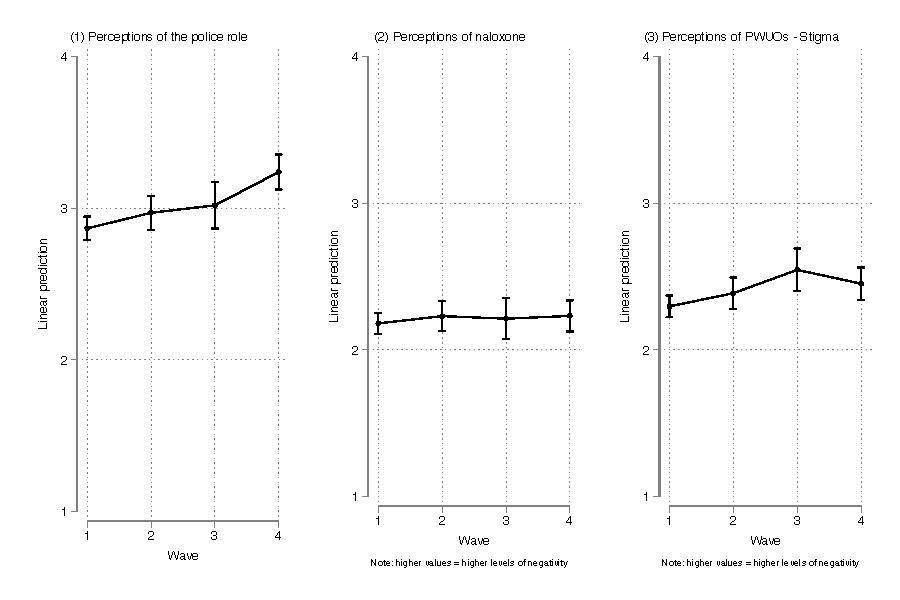
\includegraphics{figures/growth_models.pdf}
\end{figure}

% growth model coefficients table
\begin{table}[htbp]\centering
\def\sym#1{\ifmmode^{#1}\else\(^{#1}\)\fi}
\caption{\centering Unconditional Linear Growth Models}
\begin{tabular}{l*{3}{c}}
\toprule
                &\multicolumn{1}{c}{(1)}&\multicolumn{1}{c}{(2)}&\multicolumn{1}{c}{(3)}\\
                &\multicolumn{1}{c}{Role of the police}&\multicolumn{1}{c}{Naloxone related beliefs}&\multicolumn{1}{c}{Stigma towards PWUOs}\\
\midrule
Wave 2          &0.103 (0.069)        &0.050 (0.063)        &0.090 (0.066)        \\
\addlinespace
Wave 3          &0.152\sym{+} (0.087)        &0.032 (0.080)        &0.249\sym{**} (0.083)        \\
\addlinespace
Wave 4          &0.372\sym{**} (0.071)        &0.051 (0.065)        &0.155\sym{*} (0.067)        \\
\addlinespace
Constant        &2.867\sym{**} (0.040)        &2.181\sym{**} (0.036)        &2.297\sym{**} (0.038)        \\
\midrule
Observations    &      527        &      525        &      527        \\
\bottomrule
\multicolumn{4}{l}{\footnotesize Standard errors in parentheses}\\
\multicolumn{4}{l}{\footnotesize \sym{+} \(p<0.10\), \sym{*} \(p<0.05\), \sym{**} \(p<0.01\)}\\
\end{tabular}
\end{table}


% pooled reg models coefficients
% add note re robust se's in model (1) + reference categories: never responding to an overdose, never administered naloxone, White, male, less than a year at the department, in wave 1.

\begin{landscape}
\begin{table}[htbp]\centering
\def\sym#1{\ifmmode^{#1}\else\(^{#1}\)\fi}
\caption{\centering Pooled OLS Regression Models}
\begin{tabular}{l*{3}{c}}
\toprule
                &\multicolumn{1}{c}{(1)}&\multicolumn{1}{c}{(2)}&\multicolumn{1}{c}{(3)}\\
                &\multicolumn{1}{c}{\hspace{0.25cm} Role of the police}&\multicolumn{1}{c}{\hspace{0.25cm} Naloxone related beliefs}&\multicolumn{1}{c}{\hspace{0.25cm} Stigma towards PWUOs}\\
\midrule
\emph{OD Response Frequency}&                  &                  &                  \\
\hspace{0.25cm} Rarely (less than once per week)&0.024 (0.082)         &-0.076 (0.076)         &-0.101 (0.078)         \\
\hspace{0.25cm} Once per week&0.000 (0.091)         &-0.005 (0.088)         &-0.069 (0.091)         \\
\hspace{0.25cm} Once per shift&0.034 (0.167)         &0.010 (0.133)         &-0.113 (0.138)         \\
\hspace{0.25cm} Multiple times per shift&-0.246 (0.262)         &0.042 (0.206)         &-0.008 (0.213)         \\
\vspace{0.1em} \emph{Control Variables}&                  &                  &                  \\
\hspace{0.25cm} Ever administered naloxone&0.190\sym{***} (0.068)         &-0.094 (0.076)         &-0.035 (0.078)         \\
\hspace{0.25cm} Patrol&-0.095 (0.066)         &0.081 (0.061)         &0.034 (0.063)         \\
\hspace{0.25cm} Black&0.220 (0.134)         &0.040 (0.134)         &-0.134 (0.139)         \\
\hspace{0.25cm} Hispanic&-0.001 (0.070)         &0.119 (0.073)         &-0.009 (0.075)         \\
\hspace{0.25cm} Other&-0.059 (0.119)         &0.096 (0.121)         &0.079 (0.125)         \\
\hspace{0.25cm} Female&0.070 (0.075)         &0.072 (0.069)         &-0.158\sym{**} (0.072)         \\
\hspace{0.25cm} College degree&-0.173\sym{***} (0.062)         &-0.054 (0.061)         &-0.030 (0.063)         \\
\hspace{0.25cm} Competence at an overdose&0.172\sym{***} (0.053)         &-0.042 (0.040)         &0.099\sym{**} (0.041)         \\
\emp{Time at Tempe PD}&                  &                  &                  \\
\hspace{0.25cm} 1-2 years&-0.137 (0.103)         &0.180 (0.145)         &-0.026 (0.150)         \\
\hspace{0.25cm} 2-5 years&-0.240\sym{**} (0.115)         &0.199 (0.133)         &0.001 (0.138)         \\
\hspace{0.25cm} 6-10 years&-0.419\sym{***} (0.114)         &0.303\sym{**} (0.133)         &0.028 (0.138)         \\
\hspace{0.25cm} 11+ years&-0.318\sym{***} (0.096)         &0.114 (0.121)         &-0.040 (0.125)         \\
\emp{Wave}      &                  &                  &                  \\
\hspace{0.25cm} Wave 2&0.012 (0.071)         &0.037 (0.070)         &0.053 (0.072)         \\
\hspace{0.25cm} Wave 3&0.046 (0.110)         &0.042 (0.094)         &0.119 (0.098)         \\
\hspace{0.25cm} Wave 4&0.051 (0.092)         &0.067 (0.090)         &0.066 (0.093)         \\
Constant        &2.901\sym{***} (0.179)         &2.130\sym{***} (0.164)         &2.153\sym{***} (0.170)         \\
\midrule
Observations    &      459         &      458         &      459         \\
\(R^{2}\)       &    0.164         &    0.050         &    0.051         \\
\bottomrule
\multicolumn{4}{l}{\footnotesize Standard errors in parentheses}\\
\multicolumn{4}{l}{\footnotesize \sym{*} \(p<0.10\), \sym{**} \(p<0.05\), \sym{***} \(p<0.01\)}\\
\end{tabular}
\end{table}
 
\end{landscape}




\begin{figure}
    \centering
    \caption{\centering Coefficient Plot: Main Models}
    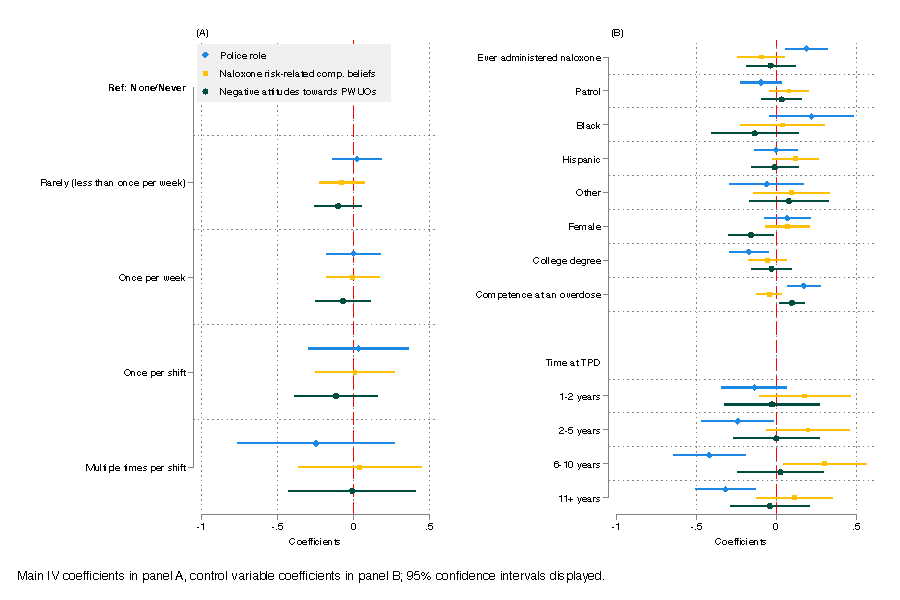
\includegraphics{figures/coefplot-combined.pdf}
\end{figure}